%%%%%%%%%%%%%%%%%%%%%%%%%%%%%%%%%%%%%%%%%%%%%%%%%%%%%%%%%%%%%%%%%%%%%%%%%%%%%%%%%%%%%%%%%%%%%%%%
%
% CS484 Written Question Template
%
% Acknowledgements:
% The original code is written by Prof. James Tompkin (james_tompkin@brown.edu).
% The second version is revised by Prof. Min H. Kim (minhkim@kaist.ac.kr).
%
% This is a LaTeX document. LaTeX is a markup language for producing
% documents. Your task is to fill out this document, then to compile
% it into a PDF document.
%
%
% TO COMPILE:
% > pdflatex thisfile.tex
%
% If you do not have LaTeX and need a LaTeX distribution:
% - Personal laptops (all common OS): www.latex-project.org/get/
% - We recommend latex compiler miktex (https://miktex.org/) for windows,
%   macTex (http://www.tug.org/mactex/) for macOS users.
%   And TeXstudio(http://www.texstudio.org/) for latex editor.
%   You should install both compiler and editor for editing latex.
%   The another option is Overleaf (https://www.overleaf.com/) which is
%   an online latex editor.
%
% If you need help with LaTeX, please come to office hours.
% Or, there is plenty of help online:
% https://en.wikibooks.org/wiki/LaTeX
%
% Good luck!
% Min and the CS484 staff
%
%%%%%%%%%%%%%%%%%%%%%%%%%%%%%%%%%%%%%%%%%%%%%%%%%%%%%%%%%%%%%%%%%%%%%%%%%%%%%%%%%%%%%%%%%%%%%%%%
%
% How to include two graphics on the same line:
%
% \includegraphics[width=0.49\linewidth]{yourgraphic1.png}
% \includegraphics[width=0.49\linewidth]{yourgraphic2.png}
%
% How to include equations:
%
% \begin{equation}
% y = mx+c
% \end{equation}
%
%%%%%%%%%%%%%%%%%%%%%%%%%%%%%%%%%%%%%%%%%%%%%%%%%%%%%%%%%%%%%%%%%%%%%%%%%%%%%%%%%%%%%%%%%%%%%%%%

\documentclass[11pt]{article}

\usepackage[english]{babel}
\usepackage[utf8]{inputenc}
\usepackage[colorlinks = true,
            linkcolor = blue,
            urlcolor  = blue]{hyperref}
\usepackage[a4paper,margin=1.5in]{geometry}
\usepackage{stackengine,graphicx}
\usepackage{fancyhdr}
\setlength{\headheight}{15pt}
\usepackage{microtype}
\usepackage{times}
\usepackage{booktabs}

% From https://ctan.org/pkg/matlab-prettifier
\usepackage[numbered,framed]{matlab-prettifier}

\frenchspacing
\setlength{\parindent}{0cm} % Default is 15pt.
\setlength{\parskip}{0.3cm plus1mm minus1mm}

\pagestyle{fancy}
\fancyhf{}
\lhead{Homework Writeup}
\rhead{CS 484}
\rfoot{\thepage}

\date{}

\title{\vspace{-1cm}Homework 2 Writeup}


\begin{document}
\maketitle
\vspace{-3cm}
\thispagestyle{fancy}

\section*{Instructions}
\begin{itemize}
  \item Describe any interesting decisions you made to write your algorithm.
  \item Show and discuss the results of your algorithm.
  \item Feel free to include code snippets, images, and equations.
  \item Use as many pages as you need, but err on the short side If you feel you only need to write a short amount to meet the brief, th

  \item \textbf{Please make this document anonymous.}
\end{itemize}

\section*{Implementing my\_imfilter}
Homework 2 starts with implementing one's own \texttt{my\_imfilter} function that partially replicates the behavior of matlab's own \texttt{imfilter} function. The algorithm operates as follows:
\begin{enumerate}
    \item Check the size of the filter
        \begin{enumerate}
            \item If the width or height of the filter is not odd, throw an error
        \end{enumerate}
    \item Rotate the filter by 180 degrees
    \item Pad the given image with zeros
    \item Compute the output pixel values of each pixel in the input
\end{enumerate}

\section*{Interesting Implementation Detail}
Since the algorithm is quite straightforward, there were not a lot of room for diversity in the implementation, but the interesting detail about my implementation is that it is simple and yet does a lot. This is highlighted in this particular code snippet:

\begin{lstlisting}[style=Matlab-editor]
for i = 1 + half_m : m - half_m
    for j = 1 + half_n : n - half_n
        for k = 1 : h
            partial = image(i - half_m:i + half_m, j - half_n:j + half_n, k);
            output(i - half_m, j - half_n, k) = sum(partial .* rotated_filter, 'all');
        end
    end
end
\end{lstlisting}

The interesting thing about this snippet is the usage of element-wise product and \texttt{sum} function in line 4. This part could have ended up being a double nested for loop, but implementing it as so makes the code cleaner and easier to read. The fact that no branches were used in order to handle two different types of images - grayscale and color, is also noteworty.

\section*{Hybrid Image Creation}
The following is the entire implementation of hybrid image creation. One thing to note in this code is that the high-pass filtered image is simply generated by subtracting the low-pass version from the original image.
\begin{lstlisting}[style=Matlab-editor]
function [hybrid_image,low_frequencies,high_frequencies] = gen_hybrid_image( image1, image2, cutoff_frequency )
% Inputs:
% - image1 -> The image from which to take the low frequencies.
% - image2 -> The image from which to take the high frequencies.
% - cutoff_frequency -> The standard deviation, in pixels, of the Gaussian
%                       blur that will remove high frequencies.
filter = fspecial('Gaussian', cutoff_frequency * 4 + 1, cutoff_frequency);
low_frequencies = my_imfilter(image1, filter);

high_frequencies = image2 - my_imfilter(image2, filter);

hybrid_image = low_frequencies + high_frequencies;
\end{lstlisting}

\section*{Result}
Upon execution of the given starter code, the results show expected, but still interesting results. Here are a few visualizations that demonstrate the results:

\begin{figure}[h]
    \centering
    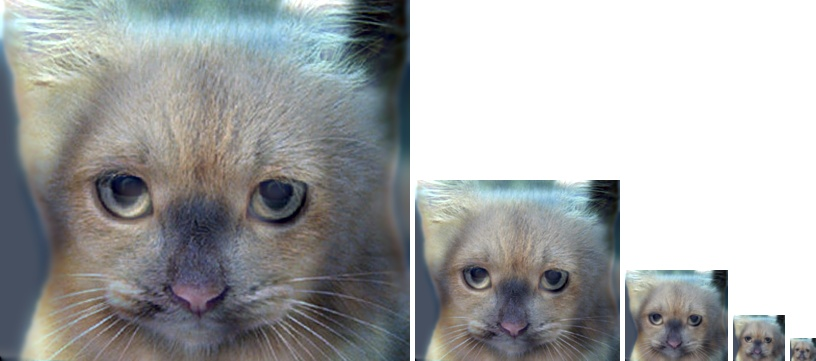
\includegraphics[width=4cm]{dog-cat.jpg}
    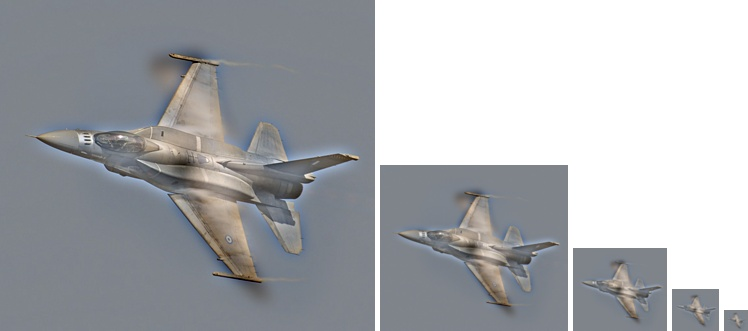
\includegraphics[width=4cm]{bird-plane.jpg}
    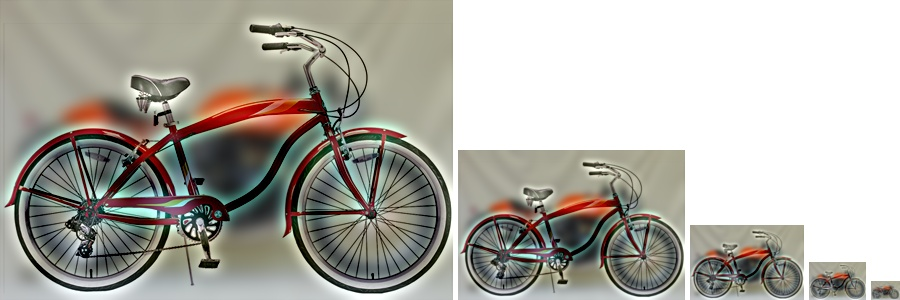
\includegraphics[width=4cm]{motorcycle-bicycle.jpg}
    \caption{\emph{Left:} Dog-Cat \emph{Middle:} Bird-Plane \emph{Right:} Motorcycle-Bicycle}
\end{figure}

Another interesting observation is that it does not always seem to be the case that certain image pairs need different cutoff values for the hybrid image to be perceived differently at different distances. Here is the hybrid image for a Cat-Dog pair(low-pass cat and high-pass dog) with the \texttt{cutoff\_frequency} value at 7.

\begin{figure}[h]
    \centering
    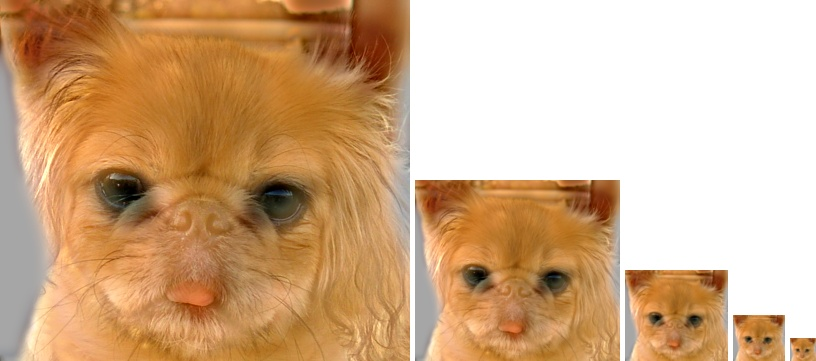
\includegraphics[width=8cm]{cat-dog.jpg}
    \caption{cat-dog hybrid image at cutoff\_frequency=7}
\end{figure}

At least in the author's perspective, although there exists a silhouette of a dog in the image when viewed closely, it does not seem to provide the same amount of effect that other hybrid images demonstrate. In an attempt to produce better results, I have raised the value of \texttt{cutoff\_frequency} to be 13.

\begin{figure}[h]
    \centering
    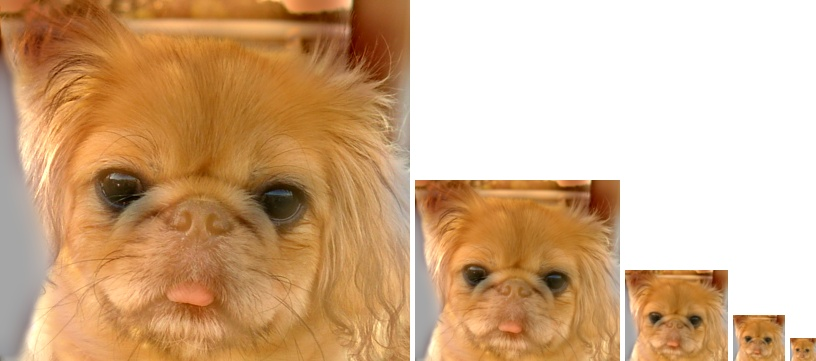
\includegraphics[width=8cm]{cat-dog-improved.jpg}
    \caption{cat-dog hybrid image at cutoff\_frequency=13}
\end{figure}

One can see that the subtle change in the cutoff frequency allows images to be better and naturally recognized as a dog when viewed from close distance.

\end{document}
